% --- Template for thesis / report with tktltiki2 class ---
% 
% last updated 2013/02/15 for tkltiki2 v1.02

\documentclass[finnish]{tktltiki2}

% tktltiki2 automatically loads babel, so you can simply
% give the language parameter (e.g. finnish, swedish, english, british) as
% a parameter for the class: \documentclass[finnish]{tktltiki2}.
% The information on title and abstract is generated automatically depending on
% the language, see below if you need to change any of these manually.
% 
% Class options:
% - grading                 -- Print labels for grading information on the front page.
% - disablelastpagecounter  -- Disables the automatic generation of page number information
%                              in the abstract. See also \numberofpagesinformation{} command below.
%
% The class also respects the following options of article class:
%   10pt, 11pt, 12pt, final, draft, oneside, twoside,
%   openright, openany, onecolumn, twocolumn, leqno, fleqn
%
% The default font size is 11pt. The paper size used is A4, other sizes are not supported.
%
% rubber: module pdftex

% --- General packages ---

\usepackage[utf8]{inputenc}
\usepackage[T1]{fontenc}
\usepackage{lmodern}
\usepackage{microtype}
\usepackage{amsfonts,amsmath,amssymb,amsthm,booktabs,color,enumitem,graphicx}
\usepackage[pdftex,hidelinks]{hyperref}

% Automatically set the PDF metadata fields
\makeatletter
\AtBeginDocument{\hypersetup{pdftitle = {\@title}, pdfauthor = {\@author}}}
\makeatother

% --- Language-related settings ---
%
% these should be modified according to your language

% babelbib for non-english bibliography using bibtex
\usepackage[fixlanguage]{babelbib}
\selectbiblanguage{finnish}

% add bibliography to the table of contents
\usepackage[nottoc]{tocbibind}
% tocbibind renames the bibliography, use the following to change it back
\settocbibname{Lähteet}

% --- Theorem environment definitions ---

\newtheorem{lau}{Lause}
\newtheorem{lem}[lau]{Lemma}
\newtheorem{kor}[lau]{Korollaari}
\theoremstyle{definition}
\newtheorem{maar}[lau]{Määritelmä}
\newtheorem{ong}{Ongelma}
\newtheorem{alg}[lau]{Algoritmi}
\newtheorem{esim}[lau]{Esimerkki}

\theoremstyle{remark}
\newtheorem*{huom}{Huomautus}


% --- tktltiki2 options ---
%
% The following commands define the information used to generate title and
% abstract pages. The following entries should be always specified:

\title{Esimerkkiotsikko}
\author{Eija Esimerkki}
\date{\today}
\level{Seminaariraportti}
\abstract{Tiivistelmä.}

% The following can be used to specify keywords and classification of the paper:

\keywords{avainsana 1, avainsana 2, avainsana 3}
\classification{} % classification according to ACM Computing Classification System (http://www.acm.org/about/class/)
                  % This is probably mostly relevant for computer scientists

% If the automatic page number counting is not working as desired in your case,
% uncomment the following to manually set the number of pages displayed in the abstract page:
%
% \numberofpagesinformation{16 sivua + 10 sivua liitteissä}
%
% If you are not a computer scientist, you will want to uncomment the following by hand and specify
% your department, faculty and subject by hand:
%
% \faculty{Matemaattis-luonnontieteellinen}
% \department{Tietojenkäsittelytieteen laitos}
% \subject{Tietojenkäsittelytiede}
%
% If you are not from the University of Helsinki, then you will most likely want to set these also:
%
% \university{Helsingin Yliopisto}
% \universitylong{HELSINGIN YLIOPISTO --- HELSINGFORS UNIVERSITET --- UNIVERSITY OF HELSINKI} % displayed on the top of the abstract page
% \city{Helsinki}
%


\begin{document}

% --- Front matter ---

\maketitle        % title page
\makeabstract     % abstract page

\tableofcontents  % table of contents
\newpage          % clear page after the table of contents


% --- Main matter ---

\section{Johdanto}

World Wide Web (WWW) tarjoaa staattisen informaation lisäksi palveluita. Web-palvelu voi yksinkertaisimmillaan palauttaa informaatiota pyynnön saatuaan tai monimutkaisemmassa tapauksessa voidaan tehdä  esimerkiksi ostos, jossa veloitetaan luottokorttia ja muodostetaan toimitettava tilaus\cite{with_owls}. 

Ohjelmoijan on varsin helppo tuottaa ohjelma, joka käyttää web-palvelua. Tekniikoita palveluiden käyttämiseen on monia, mutta yleinen tapa on lähettää palvelulle viesti, joka on koodattu sovitulla tavalla, esimerkiksi XML:llä tai Jsonilla. Erilaiset datatyypit ja viestien (ja niiden osien) muodot voidaan  selostaa esimerkikisi WSDL-dokumentissa \cite{WSDL}. Edellä mainittujen tekniikoiden toteuttaminen ei nykyaikaisilla ohjelmistokirjastiolle ja IDE:illä ole edes monimutkaista. Mutta olipa tekniikka mikä tahansa, tässä muodossa palvelun käyttö vaatii aina \textit{ihmisen} puuttumisen asiaan. \textit{ihminen} on se, joka hakee palvelun. \textit{ihminen} on se, joka tutkii palvelun kuvauksen ja muokkaa oman ohjelmansa (tai palvelun) käyttämään sitä. 

Mutta mitä \textit{emme} voi löytää WSDL-kuvauksesta, on se, mitä palvelussa tapahtuu, kun sitä käytetään\cite{with_owls}. Jotta voidaan välttää ihmisen osallistumien web-palvelujen orkestrointiin, tulee olla \textit{automaattisia ohjelmistoagentteja}, jotka etsivät oikeat palvelut ja käyttävät niitä automaattisesti, ilman ihmisen puuttumista asiaan\cite{with_owls}.

Automaattinen ohjelmistoagentti mahdollistaisi esimerkiksi:

\begin{itemize}
\item \textit{Presentaation pitäjä haluaa lähettää esitysmateriaalinsa kaikkien osanottajien käyttöön. Hän voisi tehdä sen yhdellä lähetysnapin painalluksella riippumatta siitä, mitä teknologioita ja protokollia vastaanottajat käyttävät}\cite{with_owls}.

\item \textit{Kuluttaja haluaa löytää haluamansa tuotteen mahdollisimman halvalla jostain verkkokauasta. Ohjelmistoagenttia hyödyntävä ohjelma hakee tuotteen hintaa ja saatavuutta useista verkkokaupoista, jotka ovat koodanneet kataloginsa jotain standardoitua sanastoa käyttäen. Sanastojen ei edes tarvitse olla samat eri verkkokaupoilla}\cite{with_owls}. 
\end{itemize}

Ohjelmistoagenteille tulisi siis pystyä antamaan tarvittava informaatio muodossa, jota se ymmärtää. \textit{Semanttinen web} voi tarjota ratkaisun tähän. Vuonna 2001 Tim Berners-Lee, James Hendler ja Ora Lassila julkaisivat artikkelin "the Semantic Web", jossa he
luonnehtivat semanttista webiä seuraavasti:
\begin{quote}
"Semanttinen web ei ole erillinen web vaan
laajennos tämänhetkiseen webiin, jossa informaatiolle on annettu hyvin muotoiltu
merkitys mahdollistaen koneiden ja ihmisten paremman yhteistyön.[suomennos kirjoittajan]\cite{semweb}
\end{quote}

Ohjelmistoagenttien tulee pystyä \textit{ymmärtämään} \textit{mitä} palveluntarjoaja tarjoaa ja \textit{miten} palvelu tuotetaan. Tunnetusti kone ei ymmärrä ihmisen ymmärtämää teksti-informaatiota. Koneelle pitää siis tarjota mahdollisuus ymmärtää käsitteitä, antaa mahdollisuus luoda uutta ymmärrystä käsitteiden ja käsitteiden välisten suhteiden pohjalta. Koneen tulee pystyä ymmärtämään \textit{semantiikoita}. 

Webissä semantiikoita ilmaistaa ontologioilla, jotka tietojenkäsittelytieteessä ymmärretään dokumentteina, joissa kerrotaan asioiden välisistä yhteyksistä\cite{semweb}. Kun web-palveluita kuvataan ontologioiden avulla, tulee käytössä olla kuvaamiseen soveltuva \textit{sanasto}, ontologia. Yksi mahdollinen tällainen sanasto on OWL-S, joka tulee sanoista Web Ontology Language for Services. OWL-S tarjoaa luokat ja ominaisuudet, joiden avulla web-palvelu voidaan kuvata koneen ymmärtämässä muodossa. Jotta voimme ymmärtää OWL-S:llä tuotettuja ontologioita, pitää ensin tutustua soveltuvin osin OWL (Web Ontology Language) :ään ja sen kostruktioihin, joiden avulla web-palveluontologioita voidaan muodostaa. 

\section{Web-ontologiakieli OWL}

World Wide Web Consortium on antanut OWL:lle suosituksen standardiksi vuonna 2004\cite{owlguide}. Uudempi suositus on OWL 2:lle vuodelta 2012. OWL kielenä perustuu muutamiin jo aiemmin määriteltyihin merkintätapoihin ja konsepteihin, kuten XML:ään ja RDF:ään ja URI:in .

\subsection{URI, XML ja RDF}

Semanttisessa webissä määritettyjä luokkia, ilmentymiä ja niiden välisiä suhetita identifioidaan URI:en avulla\cite{semweb}.
URI (Uniform Resource Identifier) on standardi resurssien identifioimiseen. Useimmiten URI:na käytetään tavallista URL:ia (Uniform Resource Locator). Identifiointi on tärkeää, koska näin pystytään erottelemaan jo luodut resurssit itse luoduista resursseista. 

XML-kieli on notaatio rakenteisen kielen esittämiseen. Useimmiten semanttisessa webissä tietoa kuvataan nimenomaan XML-tiedostoina, koska ne ovat helposti koneen tulkittavissa. XML:n nimiavaruudet helpottavat resurssien identifioimista URI:en avulla. 

RDF (Resource Description Framework) on yksinkertainen tapa kuvailla webissä olevaa tietoa kolmikoiden avulla\cite{RDFP}. RDF-kolmikon muodostavat subjekti, objekti ja predikaatti\cite{RDFP}. Subjekti on asia, jota kuvataan, predikaatti on ominaisuus, jolla asiaa kuvataan ja objekti on ominaisuuden arvo. Esimerkiksi tieto ''Matin veli on Teppo'' voidaan kuvata kolmikolla 


ESIMERKKI


Esimerkistä voimme havaita, että kuvailtava asia on subjekti nimeltään \textit{matti}, jota kuvataan suhteella \textit{veli} joka saa arvokseen \textit{teppo}. Tämänkaltainen XML-kielinen notaatio on OWL:n (ja OWL-S:n) ontologioiden kuvaamisen syntaktinen ydin. Pelkkä RDF -syntaksi ei kuitenkaan riitä, koska ontologioiden (semantiikoiden) kuvaamiseen tarvitaan myös monimutkaisempia abstraktioita, kuten \textit{luokka}, \textit{aliluokka}, \textit{ilmentymä}, \textit{suhde} ja \textit{alisuhde}. Nämä konstruktiot tarjoaa RDF:n semanttinen laajennos RDF Schema (RDFS) sekä OWL, joka käyttää suurta osaa RDFS:n konstruktioita lähes sellaisenaan.  

\subsection{Tarpeelliset OWL- ja RDFS -konstruktiot OWL-S:n ymmärtämiseen}

OWL on kehittynyt versio RDF Schemasta. 



luokka

instanssi

suhde

aliluokka

alisuhde

import

union

disjointWith

risuaitaviittaukset


\section{Webpalveluiden kuvauskieli OWL-S}

UDDI löytäminen, käyttö, monitorointi

\subsection{Korkean abstraktiotason rakenne}

Palveluontologian korkean abstraktiotason rakenne muodostuu kolmen tyyppisestä tiedosta ja ne vastaavat kolmeen eri kysymykseen \cite{OWLS}:

\begin{itemize}

  \item \textit{Mitä palvelu tarjoaa mahdolliselle asiakkaalle?} Tähän antaa vastauksen ontologian \textit{profiili}, joka kertoo karkealla tasolla mitä palvelu tarjoaa. Profiilin 
 avulla palveluntarjoaja voi mainostaa palveluaan potentiaalisille asiakkaille. Profiilissa kerrotan myös, \textit{kuka} palvelun tarjoaa. Jokainen \texttt{Service}-luokka edustaa yhtä \texttt{ServiceProfilea} \cite{OWLS}.
 
 \item \textit{Kuinka palvelua käytetään?} Ontologian \textit{prosessimalli} antaa vastauksen tähän ja se esitetään luokassa \texttt{ServiceModel}. Palvelun ja sen prosessimallin 
 välillä on \texttt{describedBy} -suhde\cite{OWLS}. 
 
 \item \textit{Miten palvelun kanssa kommunikoidaan?} Tähän antaa vastauksen ontologian \textit{maadoitus}, jossa määritellään esimerkiksi tuki erilaisille viestiprotokollille. 
 \texttt{Service} -luokalla on ominaisuus \texttt{supports}, joka viittaa \texttt{ServiceGrounding} -luokkaan\cite{OWLS}.  
 
 \begin{figure}[ht]
 \centering
 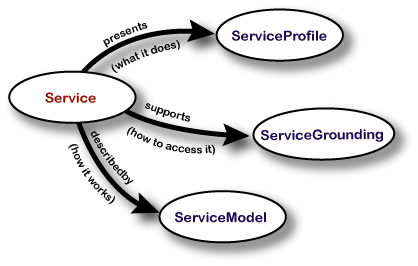
\includegraphics[scale=0.60]{karkea_taso.png}
 \caption{OWL-S:llä kuvatun palveluontologian korkean taon rakenne \cite{OWLS}}
 \label{karkea_taso}
\end{figure}
 
 Kuten kuvasta \ref{karkea_taso}  voidaan nähdä, jokaista julkistettua palvelua kohden on yksi \texttt{Service}-luokan instanssi, joka edustaa \texttt{ServiceProfilea} suhteella \texttt{presents}, on \texttt{ServiceModel}in kuvailema suhteella \texttt{describedBy} ja \texttt{serviceGrounding}in tukema suhteella \texttt{supports}.
 
\end{itemize}


\subsection{Profiili}

Profiili siis kertoo mitä palvelu tekee ja kuka palvelun tarjoaa. Se mahdollistaa asiakkaita (agentteja) löytämään palvelun esimerkikisi keskitetyistä palvelurekistereistä kuten UDDI tai puhtaan P2P:n puitteissa. 
Profiili tarjoaa kolmenlaista informaatiota \cite{OWLS}:

\begin{enumerate}
 \item \textit{Tuottajainformaatio} kertoo tietoja palvelun tuottajasta, esimerkiksi ylläpitäjän tai asiakasyhteyshenkilön yhteystiedot. Myös lyhyt tekstikuvaus palvelusta sekä yksikäsitteinen nimi palvelulle määritellään profiilissa\cite{OWLS} .
 
 \item \textit{Toiminnallinen kuvaus} kuvaa (tautologia) palvelun käyttämät \textit{syötteet}, sen tuottamat \textit{tulosteet}, \textit{esiehdot}, jotka tulee olla voimassa ennen määrättyjä
 prosesseja sekä \textit{tilamuutoksia}, joita prosessien suorittaminen aiheuttaa \cite{OWLS}. ESIMERKKEJÄ?? Nämä samat käsitellään myös prosessimallissa, mutta tarkemmalla tasolla. OWL-S ei aseta
 rajoitteita sen suhteen, onko profiili ja prosessimalli konsistentit toisiinsa nähden, mutta ollakseen totuudenmukainen palvelun tarjoamien todellisten palvelujen suhteen, tulee profiilin ilmaista
 palvelut yhtenevästi prosessimallin suhteen. 
 
 \item \textit{Toimintaa kuvaavat ominaisuudet} ?? Ensinnäkin palvelu voidaan luokitella jonkun tunnetun luokittelun, esimerkiksi UNSPSC:n [footnote] mukaan. Toiseksi, palvelun laatuluokitus voidaan 
 ilmaista profiilissa. Profiilin lopussa on määrittelemätön määrä parametreja, joilla voidaan kertoa esimerkiksi palvelun maantieteellisestä saatavuudesta, arvioidusta vasteajasta jne. \cite{OWLS}.
\end{enumerate}

Seuraavassa käsitellään em. kolmea osa-aluetta sekä profiilitiedoston rakenne tarkemmin. 

\subsubsection{Ontologioiden tuonti ja viitteet prosessimalliin sekä palveluun}

Profiilin(-tiedoston) alussa voidaan tuoda ontologian käyttöön muita jo määriteltyjä ontologioita tavallisilla owl:n \texttt{imports}-lauseilla. Esimerkissä tuodaan palvelun pääasiallinen määritelmä \texttt{BravoAirService} ontologian käyttöön\cite{daml}:  

\begin{verbatim}
<owl:imports rdf:resource="http://www.daml.org/services/owl-s/1.2/BravoAirService.owl"/>
\end{verbatim} 

Jokaista profiilia edustaa palvelu. Viittaus palvelun määritelmään ilmaistaan \texttt{presentedBy}-suhteella\cite{daml}: 

\begin{verbatim}
<service:presentedBy rdf:resource="http://www.daml.org/services/owl-s/1.2/BravoAirService.owl#BravoAir_ReservationAgent"/> 
\end{verbatim} 

\subsubsection{Tuottajainformaatio}

Palveluntarjoajan yhteystiedot on tarkoitettu pääasiassa ihmisten luettavaksi. Yhteyshenkilöitä voidaan luonnollisestikin määritellä useita, esimerkissä ainoastaan yksi\cite{daml}:  

\begin{verbatim}
<profile:contactInformation>
  <actor:Actor rdf:ID="BravoAir-reservation">
  <actor:name>BravoAir Reservation department</actor:name>
  <actor:title>Reservation Representative</actor:title>
  <actor:phone>412 268 8780</actor:phone>
      . . .
  </actor:Actor>
</profile:contactInformation>
\end{verbatim} 

Yteystietoihin kirjataan usein ylläpitäjän ja/tai kaupallisen edustajan tietoja. 

Palvelun tekstikuvaus kirjoitetaan \texttt{textDescription}-tägin ja nimi \texttt{serviceName}-tägin sisään.  


\subsubsection{Toiminnallinen kuvaus}

Toiminnallinen kuvaus ilmaisee mitä toimintoja palvelu tarjoaa ja minkä ehtojen puitteissa. OWL-S \texttt{Profile} ilmaisee kahdenlaista funktionaalisuutta: syötteet ja tulosteet, jotka voidaan ajatella informaatiovirtoina sekä esiehdot ja vaikutukset, jotka voidaan ajatella tilamuutoksina. Edellisiä vastaavat owl-ominaisuudet ovat\cite{OWLS}:

\textbf{hasInput}, joka saa arvokseen \texttt{Process}-ontologiassa määriteltyjä \texttt{Input}-luokan ilmentymiä. 


\textbf{hasOutput}, joka saa arvokseen \texttt{Process}-ontologiassa määriteltyjä \texttt{Output}-luokan ilmentymiä


\textbf{hasPrecondition}, joka määrittelee jonkin esiehdon, joka on luokan \texttt{Precondition} ilmentymä


\textbf{hasresult}, joka ilmaisee minkä ehtojen puitteissa tuloksia generoidaan sekä ja mitä tilamuutoksia prosessien suoritus saa aikaan. Saa arvokseen \texttt{Result}-luokan ilmentymiä.  

Alla olevassa esimerkissä on määritetty, että prosessilla on syöte ''lähtökenttä'' (\textit{departureAirport}), tuloste ''lentoja löytynyt'' (\textit{FlightsFound}) ja 
tilamuutos ''istumapaikka löytynyt'' (\textit{HaveSeatResult})\cite{daml}:

\begin{verbatim}
 <profile:hasInput rdf:resource="http://www.daml.org/services/owl-s/1.2/BravoAirProcess.owl#DepartureAirport"/
 <profile:hasOutput rdf:resource="http://www.daml.org/services/owl-s/1.2/BravoAirProcess.owl#FlightsFound"/>
 <profile:hasResult rdf:resource="http://www.daml.org/services/owl-s/1.2/BravoAirProcess.owl#HaveSeatResult"/
\end{verbatim}

Edellisessä esimerkissä on poimittu ainoastaan muutamia toiminnallisia määrityksiä, todelliset määritykset voi katsoa liitteestä nnn. 

\subsubsection{Toimintaa kuvaavat ominaisuudet}

Edellisessä aliluvussa luettelimme palvelun toiminnallisia ominaisuuksia.

Ontologiassa on myös mahdollista ilmoittaa palvelun luokitus jossain ontologiassa määriteltyä, mahdollisesti ulkopuolista luokitusta tai taksonomiaa käyttäen. Luokitus ilmaistaan \texttt{serviceCategory}-tagien sisällä ja arvo on \texttt{ServiceCategory}-luokan ilmentymän.  \texttt{ServiceCategory} luokalla on ominaisuuksia kategorian nimen, koodin jne ilmaisuun\cite{OWLS}. ESIMERKKI?

Profiilissa voidaan myös ilmaista palvelun tarjoajan tärkeäksi kokemia vapaavalintaisia attribuutteja \texttt{serviceParameter}-ominaisuudella. Parametrille annetaan aina nimi, joka on datatyyppiominaisuus sekä arvo, joka on jonkin olion instanssi\cite{OWLS}. Esimerkiksi palvelulle voidaan määritellä ominaisuus ''BravoAir Geographic Radius'' ja se saa arvoksen ontologiassa määritetyn alueen \texttt{jenkkilä}.

SERVICE CLASsIFICATION JA SERVICE PRODUCT?

\subsection{Prosessi}

Jotta voidaan tarjota yksityiskohtaista tietoa siitä, miten olla vuorovaikutuksessa palvelun kanssa, esitetään se OWL-S:ssä myös \textit{prosessina}. On tärkeää tietää, että prosessimalli ei ole suortettava ojelma, vaan ainoastaan kuvaus siitä\cite{OWLS}. Se kertoo, kuinka asiakasohjelmisto voi kommunikoida palvelun kanssa. 

Prosessikuvaukset jaetaan kolmeen kategoriaan\cite{OWLS}:
\begin{enumerate}
\item \textit{atominen prosessi} on sellaisen prosessin kuvaus, joka ottaa vastaan yhden viestin ja palautta yhden viestin. 
\item \textit{komposiittiprosessi} kuvaa prosessia, joka koostuu useasta eri atomisesta prosessista, ja joka ylläpitää tilatietoa. 
\item \textit{yksinkertainen prosessi} ei ole suoritettavissa eikä se kytkeydy maadoitukseen. Sen rooli on on toimia abstraktiona atomisille prosesseille tai komposiittiprosessien yksinkertaistuksena. 
\end{enumerate}

Prosesseilla voi olla määräämätön määrä syötteitä ja tulosteita. Samoin prosesseilla voi olla määräämätön määrä esiehtoja, joiden täytyy toteutua, jotta prosessi voidaan suorittaa. Vastaavasti voi olla määräämätön määrä vaikutuksia, joita prosessi aiheuttaa\cite{OWLS}.

ESIMERKKI ATMICEISTA JA KOMPOSIITEISTÄ

Seuraavassa käydään läpi prosessin kuvausta jälleen BravoAir-esimerkin\cite{daml} avulla.

\subsubsection{Osapuolet}

Prosessilla on ainakin kaksi osapuolta (participant): asiakas (client) tai tai palvelin (server). Asiakas käyttää palvelimen tarjoamia palveluja\cite{OWLS}.
Jos prosessilla on myös muita osapuolia, ne ilmaistaan \texttt{hasParticipant} suhteen avulla:
ESIMERKKI? prosessi - hasParticipant - osapuoli

\subsubsection{Syötteet ja tulosteet}

Syötteet kuvaavat prosessin sisään tuleva tietoa\cite{OWLS}. Atomisilla prosesseilla syöte on asiakkaan antama kun taas komposiittiprosesseilla osa syötteistä on asiakkaalta ja osa proessin edeltävän vaiheen tuottamaa. 

Vaikka atomisille prosesseille sallitaan ainoastaan yksi syöte, se voi todellisuudessa koostua useasta syötteestä, koska syötteitä voi BUNDLATA yhdeksi \cite{OWLS}. Tällöin pitää ymmärtää käsite \textit{viesti}, joka on usean syötteen BUNDLATTU kokonaisuus. BUNDLAUS määritellään palvelun maadoituksessa luvussa nnn. 

BravoAirin prosessikuvauksessa on atominen prosessi \texttt{SelectAvailableFlight}, joka kuvaa prosessin, jossa asiakas valitsee haluamansa lennon saatavilla olevista vaihtoehdoista \cite{daml}. Sillä on on yksi syöte, lista tarjolla olevista lennoista (\textit{SelectAvailableFlight\_FlightsAvailable}), sekä yksi paluuarvo, valittu lento (\textit{SelectAvailableFlight\_SelectedFlight}). Syöte määritellään \textit{hasInput}-tägien sisällä ja vastaavasti paluuarvo \textit{hasOutput} -tägien sisässä\cite{daml}:

\
\begin{verbatim}
<process:AtomicProcess rdf:ID="SelectAvailableFlight">
    <rdfs:label>SelectAvailableFlight (ATOMIC)</rdfs:label>
        <rdfs:comment>
            Get users prefered flight choice from available itineraries
        </rdfs:comment>
        <process:hasInput>
            <process:Input rdf:ID="SelectAvailableFlight_FlightsAvailable">
                <process:parameterType rdf:datatype="http://www.w3.org/2001/XMLSchema#anyURI">
                    http://www.daml.org/services/owl-s/1.2/Concepts.owl#FlightList
                </process:parameterType>
            </process:Input>
        </process:hasInput>
        <process:hasOutput>
            <process:Output rdf:ID="SelectAvailableFlight_SelectedFlight">
                <process:parameterType rdf:datatype="http://www.w3.org/2001/XMLSchema#anyURI">
                    http://www.daml.org/services/owl-s/1.2/Concepts.owl#FlightItineraryList
                </process:parameterType>
            </process:Output>
        </process:hasOutput>
</process:AtomicProcess>
\end{verbatim}


Esimerkissä määritellään atominen prosessi tunnuksella \texttt{SelectAvailableFlight}. Sillä on yksi syöte, joka on tyypiltään XMLSchemassa määritelty  URI ja arvoltaan lista lennoista (\texttt{Concepts.owl\#FlightList}) sekä yksi paluuarvo, joka on samaa tyyppiä ja arvoltaan valittu lento (\texttt{Concepts.owl\#FlightItineraryList}). 


\subsubsection{Esiehdot ja tulokset}

Prosessia ei voi suorittaa, jos sille määrätty esiehto ei täyty\cite{OWLS}. Esiehto on prosessin ominaisuus ja se saa arvokseen lausekkeen (\textit{expression}). ESIMERKKI?

Prosessin onnistuminen voi aiheuttaa muutoksen mailman tilassa tai sen, että palvelun kutsuja saa jotain informaatiota palvelulta. Tulos ilmaistaan termillä \textit{Result} ja se liittyy prosessiin ominaisuudella \textit{hasResult}. OWL-S:ssä ei sidota tulosta erikseen paluuarvoon tai muutokseen tilassa, vaan se määritellään \textit{Result}in sisällä\cite{OWLS}. 

Seuraavassa aliluvussa käydään läpi koko tuloksen muodostus.

\subsubsection{Ehdollisten palautusarvojen ja vaikutusten kuvaus}

Kun tulos (\texttt{Result}) on määritelty, prosessimalli voi kuvailla sitä neljällä eri ominaisuudella\cite{OWLS}: \texttt{inCondition}, \texttt{hasResultVar}, \texttt{withOutput} ja \texttt{hasEffect}\cite{OWLS}.  

\texttt{inCondition} kertoo ehdon jonka vallitessa joku tulos on mahdollinen (eikä joku toinen tulos). 

\texttt{withOutput} ja \texttt{hasEffect} puolestaan määrittelevät mitä seuraa siitä, että ehto on tosi. \texttt{hasResultVar} esittelee muuttujat, jotka sidotaan \texttt{inCondition}in määrittelemään ehtoon.  Näitä muuttujia käytetään myös tulosten muodostamiseen\cite{OWLS}. 

Seuraavassa esimerkissä esitetään tuloksen muodostuminen \cite{daml}. Esimerkki liitty prosessiin, jossa varataan lento. \texttt{hasResult} kuvaa tuloksen muodostuksen, jossa onnistuneen ostotapahtuman jälkeen palautetaan paluuarvona lentosuunnitelma (\texttt{\#BookFlight\_PreferredFlightItinerary"}) sekä varaustunnus (\texttt{\#BookFlight\_ReservationID}). 

\begin{verbatim}
<process:hasResult>
    <process:Result>
        <process:inCondition rdf:resource=
        "http://www.daml.org/services/owl-s/1.2/generic/Expression.owl#AlwaysTrue"/>
            <process:withOutput>
                <process:OutputBinding>
                    <process:toParam rdf:resource=
                        "#BookFlight_PreferredFlightItinerary"/>
                     <process:valueSource>
                          <process:ValueOf>
                              <process:theVar rdf:resource=
                                  "#CompleteReservation_PreferredFlightItinerary"/>
                              <process:fromProcess rdf:resource=
                                  "#PerformCompleteReservation"/>
                          </process:ValueOf>
                     </process:valueSource>
                 </process:OutputBinding>
             </process:withOutput>
             <process:withOutput>
                 <process:OutputBinding>
                     <process:toParam rdf:resource="#BookFlight_ReservationID"/>
                     <process:valueSource>
                         <process:ValueOf>
                             <process:theVar rdf:resource=
                                 "#CompleteReservation_ReservationID"/>
                             <process:fromProcess rdf:resource=
                                 "#PerformCompleteReservation"/>
                         </process:ValueOf>
                     </process:valueSource>
                 </process:OutputBinding>
             </process:withOutput>
    </process:Result>
</process:hasResult>
\end{verbatim}


Esimerkissä ilmaistaan ominaisuudella \texttt{inCondition} ehto, jolla kyseinen tulos muodostetaan. Tässä tapauksessa ehto on aina tosi, mikä tarkoittaa, että kyseisen prosessin suorituksessa tämä tulos muodostetaan aina. \texttt{withOutput}-ominaisuuksilla kuvataan kuinka paluuarvot sidotaan muuttujiin. Tämä tuo mukaan OWL-S:n datavuoaspektin. 

OWL-S:ssä datavuo toimii periaatteella ''kuluttaja pyytää'', eli mikään prosessi (tuottaja) ei työnnä dataa toiselle prosessille (kuluttaja) vaan kuluttajaprosessi pyytää sitä kuten esimerkkitapauksessamme \texttt{OutputBinding} -oliossa. Esimerkissä ylemmän \texttt{OutputBinding}in \texttt{toParam} -ominaisuuden arvo kertoo, että sidomme palautettavan arvon paluuarvomuuttujaan \textit{\#BookFlight\_PreferredFlightItinerary}. Muuttujan saama arvo määrätään tulevaksi prosessin  \texttt{\#PerformCompleteReservation} muuttujasta \texttt{\#CompleteReservation\_PreferredFlightItinerary}. 

Yksinkertaistettuna datavuo prosessilta prosessille kulkee seuraavalla tavalla: 

Prosessilla \textit{p2} on paluuarvomuuttujan määritys (\texttt{toParam}) nimeltään ''o2''. Määritellään, että kyseisen paluuarvomuuttujan arvo saadaan prosessin (\texttt{fromProcess} ) \textit{p1} muuttujasta (\texttt{theVar}) ''\textit{o1}''.  

KUVA!!!

\subsubsection{Komposiittiprosessit ja kontrollirakenteet}

Komposiittiprosessi voidaan hajoittaa atomisiksi prosesseiksi tai komposiittiprosesseiksi\cite{OWLS}. Tämä hajoittaminen voidaan ilmaista kontrollirakenteilla kuten \texttt{Sequence} tai \texttt{If-Then-Else}. Vaikka kontrollirakenteen nimet muistuttavat ohjelmointikielistä tuttuja nimityksiä, on syytä muistaa, että ne \textit{eivät kerro} kuinka niiden kuvaam palvelu toimii vaan miten se \textit{mahdollisesti} toimii\cite{OWLS}. 

OWL-S määrittelee luokan \texttt{compositeProcess}, jolla on tasan yksi \texttt{composedOf} -ominaisuus, joka saa arvokseen \texttt{ControlConstruct} - luokan ilmentymän. Jokaisella \texttt{ControlConstruct}:lla on ominaisuus \texttt{components}, joka saa arvokseen toisia kontrollirakenteita\cite{OWLS}. Kontrollirakenteet muodostavat siis puumaisen rakenteen, jonka solmut, jotka eivät ole lehtiä, ovat kontrollirakenteita. Puun lehdet ovat prosessien suoritusta kuvaavia luokkia nimeltään \texttt{Perform}. Jokaisella \texttt{Perform} -luokalla on ominaisuus \texttt{process}, joka viittaa suoritettavaan prosessiin\cite{OWLS}.  Prosessin saamat syötteet määräävät, koska se suoritetaan osana suurempaa kontrollirakennetta. Datavuohon palataan tarkemmin seuraavassa kappaleessa.

Komposiittirakennetta voidaan voidaan ajatella ''black boxina'', jolloin se voidaan nähdä abstraktina yksinkertaisena prosessina (\textit{simple process}). Vastaavasti yksinkertainen prosessi voidaan nähdä komposiittirakenteena, ''white boxina'' \cite{OWLS}. 

Seuraavassa luetellaan OWL-S:n kontrollirakenteita lyhyiden selostusten kera:      
 
 \begin{itemize}
\item \textbf{Sequence} on lista kontrollirakenteita, jotka suoritetaan sarjana. 
\item \textbf{Split} mahdollistaa prosessien suorituksen rinnakkaisesti. Rakenteet poimitaan kontrollirakennesäiliöstä, \texttt{ControlConstructBag}istä.
\item \textbf{Split+Join} toimii samoin kuin Sequence, mutta prosessien suorituksen jälkeen suoritetaan puomisynkronointi. Myös tässä prosessit poimitaan säiliöstä. 
\item \textbf{Any-Order} -rakenne mahdollistaa prosessien suorituksen määräämättömässä järjestyksessä mutta ei samanaikaiseti. 
\item \textbf{Choice} toimii siten, että poimitaan joku yksi säiliön prosessi suoritettavaksi.
\item \textbf{If-ThenElse} -luokassa on ominaisuus \texttt{ifCondition}, jolle annetaan ehto \texttt{Condition}. Jos ehto on tosi, suoritetaan \texttt{Else} -ominaisuuden arvona oleva kontrollirakenne tai prosessi, jos epätosi, suoritetaan \texttt{Else} -ominaisuuden arvona oleva rakenne tai prosessi. 
\item \textbf{Repeat-While ja Repeat-Until} luokat ovate luokan \texttt{Iterate} aliluokkia. Ne toimivat samaan tapaan kuin perinteisten proseduraalisten kielten while- ja do-while -rakenteet.   
\end{itemize}

\subsection{Maadoitus}

Palvelun maadoitus kertoo (grounding) kuinka palvelu on saavutettavissa käytännön tasolla. Tärkeimmät maadoitusdokumentin ilmaisemat asiat ovat viestien muoto, viestiprotokollat, sarjallistaminen, osoitteet jne\cite{OWLS}. Voidaan ajatella, että palvelun käytön abstrakti kuvaus MÄPÄTÄÄN  konkreettiselle, käytännön tasolle\cite{OWLS}. 

OWL-S:n maadoituksen tärkein tehtävä on kertoa kuinka atomisten prosessien syötteet ja paluuarvot muutetaan viesteiksi, jotka voidaan kuljettaa jollain menetelmällä, esim. html-protokollan avulla \cite{OWLS}. 

%:
OWL-S nojaa viestien määrittelyssä vahvasti jo olemassa olevaan WSDL -kieleen, jonka puitteissa on tehty paljon kehitystyötä konkreettisen viestinmäärittelyn aikaansaamiseksi. WSDL tulee sanoista Web Services Description Language ja on XML-formaatti web-palveluiden kuvaamiseksi ENDPOINTEINA, jotka käsittelevät viestejä. WSDL:ssä ENDPOINTIT ja viestit määritellään abstraktilla tasolla, mutta MÄPÄTÄÄN konkreettisiksi viestiprotokolliksi ja viestiformaateiksi \cite{WSDL}    

WSDL:n sopivuus perustuu siihen, että OWL-S:n maadoitus on melko yhdenmukainen WSDL:n \textit{sitomisen} kanssa\cite{OWLS}. Kuitenkin molempia kieliä pitää käyttää toisiaan täydentävästi, koska kumpikaan ei yksinään tarjoa kaikkia ominaisuuksia. 

%\subsubsection{Grounding }

Koska maadoituksen tarkoituksena on MÄPÄTÄ abstrakti kuvaus konkreettisiksi viestinkuljetusoperatioiksi, tulee muodostaa ikään kuin silta OWLS-n ja WSDL:n välille. Siltana toimii OWL-S:n maadoitusdokumentti. \texttt{Grounding} -luokan aliluokan \texttt{WSDLGrounding} ilmentymässä kuvataan \texttt{WSDLAtomicProcessGrounding} -ilmentymiä. Näissä em. ilmentymissä märitellään viitteet OWL-S:n  prosesseista, syötteistä ja paluuarvoista WSDL:n vastaaviin, konkreettisiin määrityksin. 

Seuraavat \texttt{WSDLAtomicProcessGrounding}in ominaisuudet MÄPPÄÄVÄT OWL-S:n konstruktioita WSDL:n vastaaviin (kaikkia ei esitelty):

\begin{itemize}
\item \texttt{wsdlDocument} kertoo käytössä olevan WSDL-dokumentin URIn. Kaikki seuraavat viittaukset wsdl-määrityksiin viittaavat tähän dokumenttiin. 

\item \texttt{wsdlOperation} viittaa wsdl-dokumentissa määriteltyyn operaatioon, joka vastaa OWL-S:n  atomista prosessia. BravoAir-esimerkissä MÄPÄTÄÄN 
prosessikuvauksessa oleva \textit{BravoAirProcess.owl\#LogIn} -prosessi WSDL-määrityksen vastaavaan operaatioon \texttt{\#LogIn\_operation}. 

\begin{verbatim}
<grounding:owlsProcess rdf:resource="http://www.daml.org/services/owl-s/1.2/BravoAirProcess.owl#LogIn"/>
<grounding:wsdlOperation rdf:resource="#LogIn_operation"/>
\end{verbatim}

WSDL:n operaatiomäärityksiä ei voi sisällyttää tähän raporttiin joten niiden rakennetta voi tutkia lähteistä \cite{daml} ja \cite{WSDL}. 

\item \texttt{wsdlInputMessage} on olio, johon on talletettu sen  WSDL-määrityksen URI, joka ilmaisee syötteitä kuljettavien viestien muodon.  

\item \texttt{wsdlInput} -oliossa MÄPÄTÄÄN jokainen mäpättävän prosessin syöte WSDL:ssä  määritetyn viestin osaksi. Ideaalitapauksessa jokaista syötettä vastaa yksi WSDL:n viestin osa. Alla olevassa esimerkissä. MÄPÄTÄÄN BravoAirin prosessikuvauksen syöte \texttt{\#LogIn\_AcctName} WSDL-määritykseen  \texttt{\#acctName}. Viittaus jälleen URI:n avulla. 
%\small
\begin{verbatim}
<grounding:wsdlInput>
    <grounding:WsdlInputMessageMap>
        <grounding:owlsParameter rdf:resource="http://www.daml.org/services/owl-s/1.2/BravoAirProcess.owl#LogIn\_AcctName"/>
        <grounding:wsdlMessagePart rdf:datatype="http://www.w3.org/2001/XMLSchema#anyURI">
            http://www.daml.org/services/owl-s/1.2/BravoAirGrounding.wsdl#acctName
        </grounding:wsdlMessagePart>
    </grounding:WsdlInputMessageMap>
</grounding:wsdlInput>
\end{verbatim}
%\normalsize

\item \texttt{wsdlOutput} ja \texttt{wsdlOutputMessage} toimivat vastaavasti kuin edelliset, mutta MÄPPÄÄVÄT prosessin paluuarvoja.
\end{itemize}


% --- Back matter ---
%
% bibtex is used to generate the bibliography. The babplain style
% will generate numeric references (e.g. [1]) appropriate for theoretical
% computer science. If you need alphanumeric references (e.g [Tur90]), use
%
% \bibliographystyle{babalpha-lf}
%
% instead.

\bibliographystyle{babplain-lf}
\bibliography{references-fi}


\end{document}
